\documentclass[12pt,a4paper, margin=1in]{article}
\usepackage{fullpage}
\usepackage{amsfonts, amsmath, pifont}
\usepackage{amsthm}
\usepackage{amsmath}
\usepackage{geometry}
\usepackage{graphicx}
\usepackage{float}
\graphicspath{{assets/}}

\geometry{
    a4paper,
    % total={210mm,297mm},
    left=10mm,
    right=10mm,
    top=5mm,
    bottom=10mm
}

\author{
    Ahmet Eren Çolak\\
    \texttt{e2587921@ceng.metu.edu.tr}
}

\title{ 
    \textbf{CENG 499 - Introduction to Machine Learning} \\ Homework 2
}

\renewcommand{\thesection}{\arabic{section}}

\begin{document}

\maketitle

\noindent\rule{19cm}{1.2pt}

\tableofcontents

\bigskip
\noindent\rule{19cm}{1.2pt}


\section{Part 1}

\subsection{KNN}

\begin{table}[H]
    \centering
    \begin{tabular}{|c|c|c|}
    \hline
    \textbf{ID} & \textbf{K} & \textbf{Similarity Metric} \\ \hline
    1           & 3          & Cosine Distance            \\ \hline
    2           & 3          & Minkowski Distance (p=2)   \\ \hline
    3           & 5          & Cosine Distance            \\ \hline
    4           & 5          & Minkowski Distance (p=2)   \\ \hline
    5           & 5          & Mahalonobis Distance       \\ \hline
    \end{tabular}
    \caption{Hyperparameter configurations}
\end{table}

I applied 10-fold cross validation 5 times for each hyperparameter configuration and plotted their accuracy's 95\% confidence intervals.

\begin{figure}[H]
    \centering
    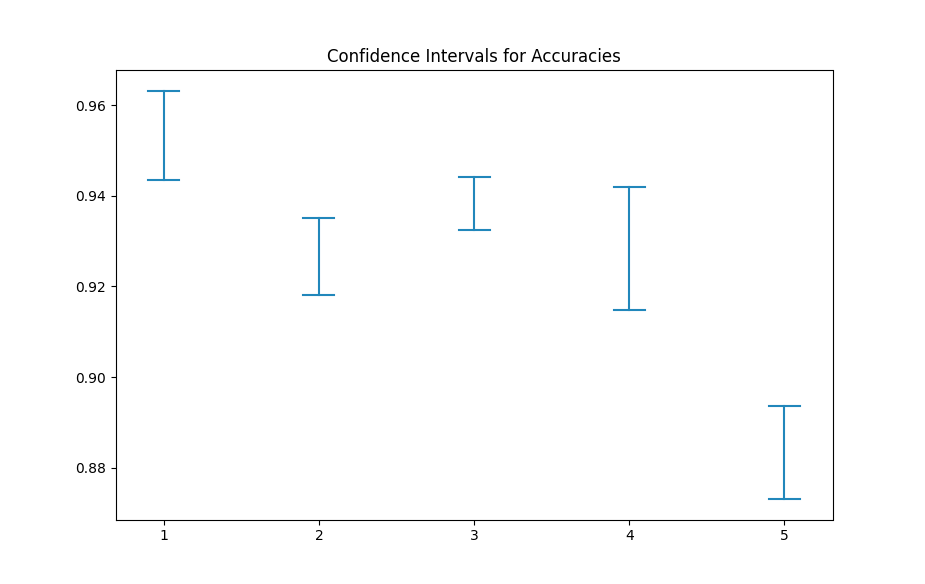
\includegraphics[scale=0.75]{confidence_intervals}
    \caption{Accuracy confidence intervals for each hyperparameter}
\end{figure}

I tested the best performing model which is the first one with $K = 3$ and cosine distance metric, with the test set which I set apart before cross validation.
Best performing model has the $\%96.67$ accuracy on the test set.

\pagebreak

\section{Part 2}

\subsection{K-Means}

I picked the initial cluster centers with K-means++ algorithm and ran K-means algorithm 10 times for each $K$ value and picked the smallest loss values for each $K$ value.

\begin{figure}[H]
    \centering
    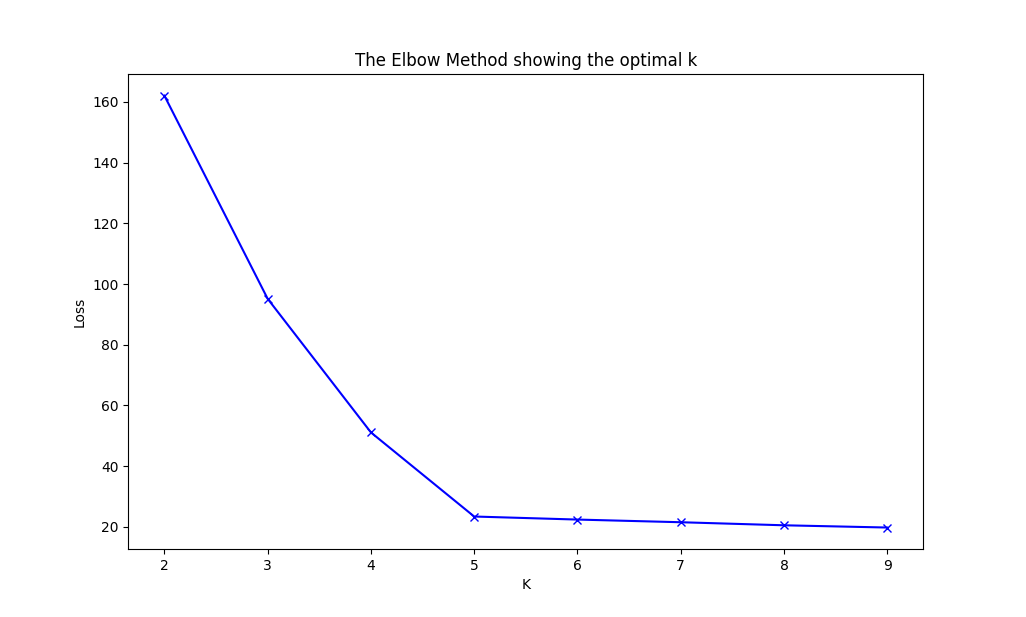
\includegraphics[scale=0.7]{elbow_dataset1}
    \caption{K vs. Loss for dataset 1}
\end{figure}

\begin{figure}[H]
    \centering
    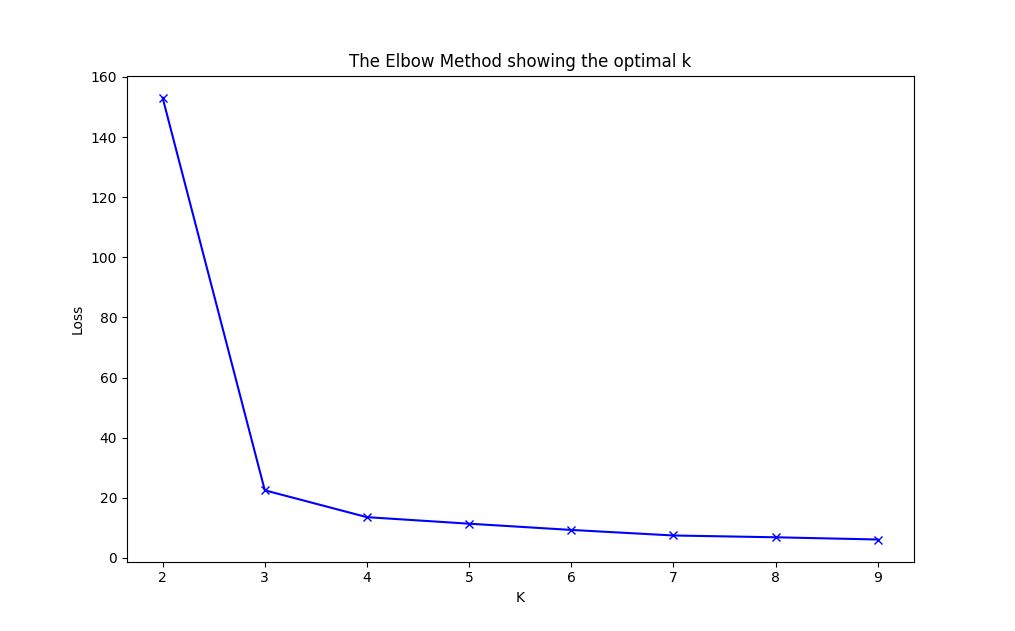
\includegraphics[scale=0.7]{elbow_dataset2}
    \caption{K vs. Loss for dataset 2}
\end{figure}

Best $K$ value for dataset 2 is $3$ and the best $K$ value for dataset 1 is $5$.

\subsection{K-Medoids}

I ran one K-medoids algorithm with cosine distance and one K-medoids algorithm with euclidean distance 10 times for each K value. Then I picked the smallest loss values for each K value.

\begin{figure}[H]
    \centering
    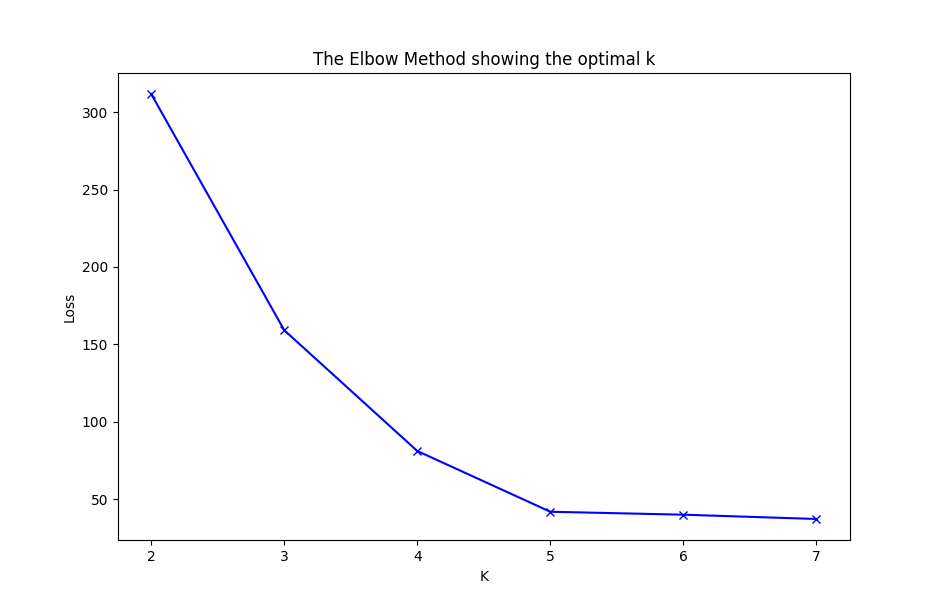
\includegraphics[scale=0.7]{elbow_kmedoids_dataset1_cosine.png}
    \caption{K vs. Loss for dataset 1 (cosine)}
\end{figure}

Best $K$ value for dataset 1 with cosine distance is $5$.

\begin{figure}[H]
    \centering
    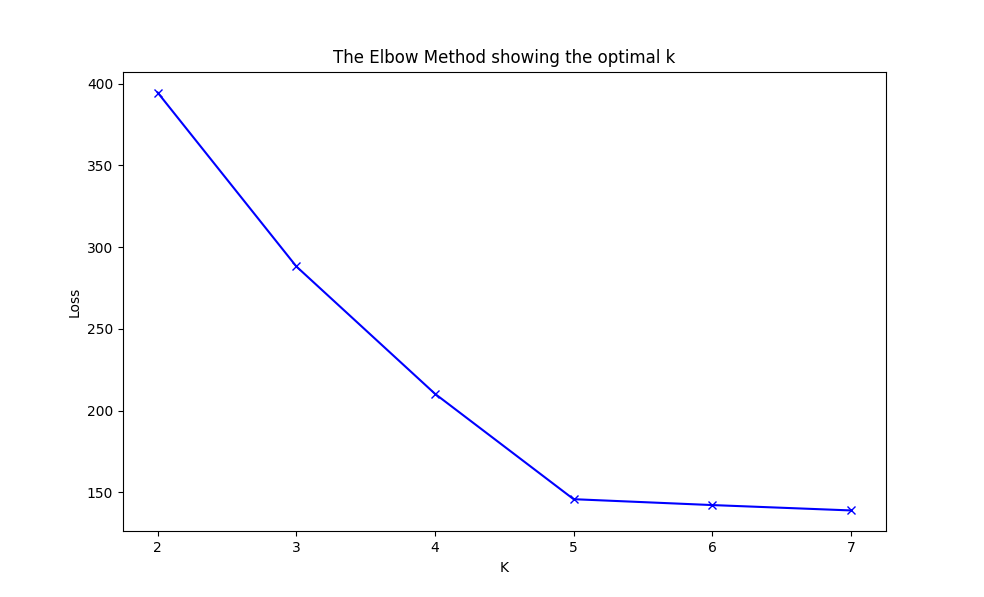
\includegraphics[scale=0.7]{elbow_kmedoids_dataset1_minkowski.png}
    \caption{K vs. Loss for dataset 1 (euclidean)}
\end{figure}

Best $K$ value for dataset 1 with euclidean distance is $5$.

\begin{figure}[H]
    \centering
    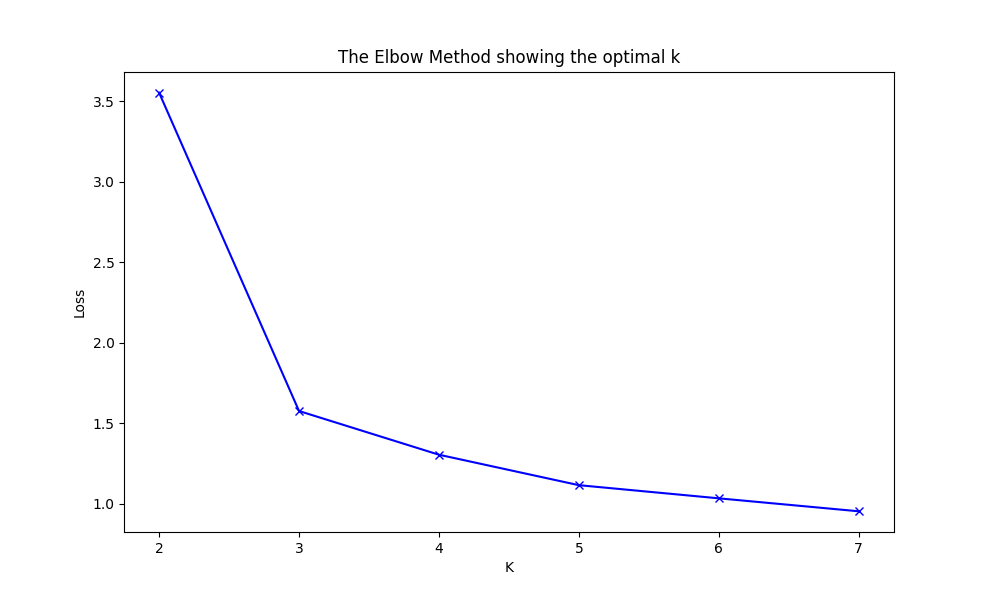
\includegraphics[scale=0.75]{elbow_kmedoids_dataset2_cosine.png}
    \caption{K vs. Loss for dataset 2 (cosine)}
\end{figure}

Best $K$ value for dataset 2 with cosine distance is $3$.

\begin{figure}[H]
    \centering
    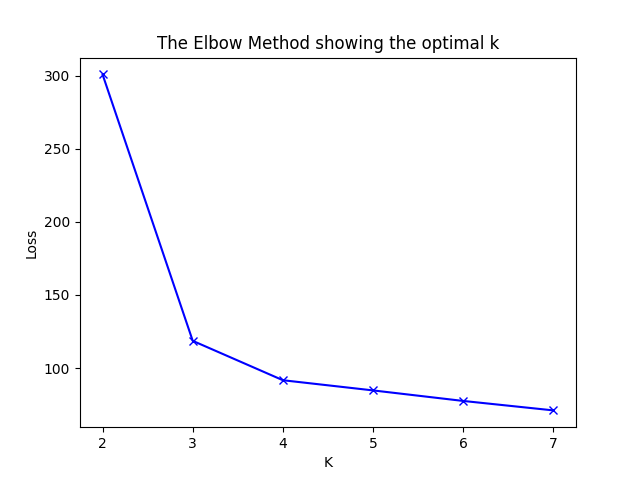
\includegraphics[scale=0.85]{elbow_kmedoids_dataset2_minkowski.png}
    \caption{K vs. Loss for dataset 2 (cosine)}
\end{figure}

Best $K$ value for dataset 2 with euclidean distance is $3$.

\subsection{2D Visualisation}

\begin{figure}[H]
    \centering
    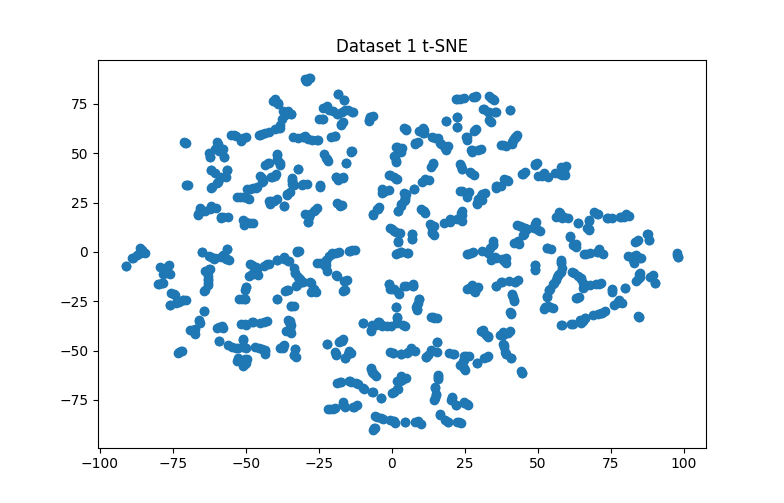
\includegraphics[scale=0.85]{dataset1_tsne.png}
    \caption{Dataset 1 dimensionality reduction with t-SNE}
\end{figure}

\begin{figure}[H]
    \centering
    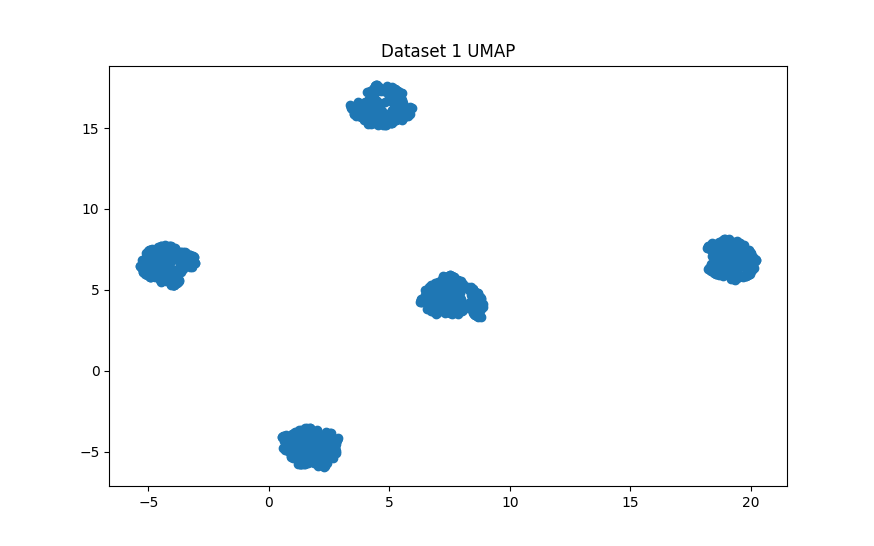
\includegraphics[scale=0.85]{dataset1_umap.png}
    \caption{Dataset 1 dimensionality reduction with UMAP}
\end{figure}

For dataset 1, optimum $K$ value obtained from elbow method and visualizations match with each other and is equal to $5$.

\begin{figure}[H]
    \centering
    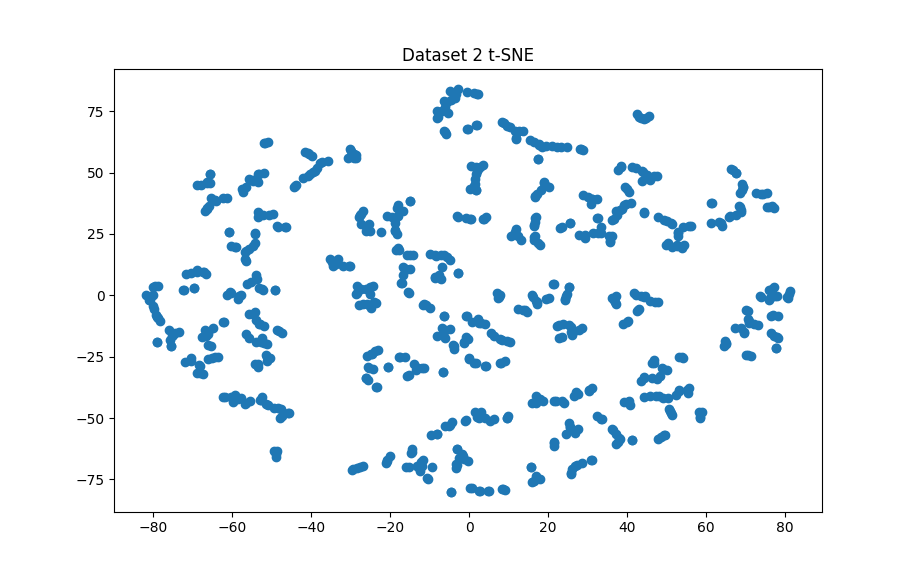
\includegraphics[scale=0.85]{dataset2_tsne.png}
    \caption{Dataset 2 dimensionality reduction with t-SNE}
\end{figure}

\begin{figure}[H]
    \centering
    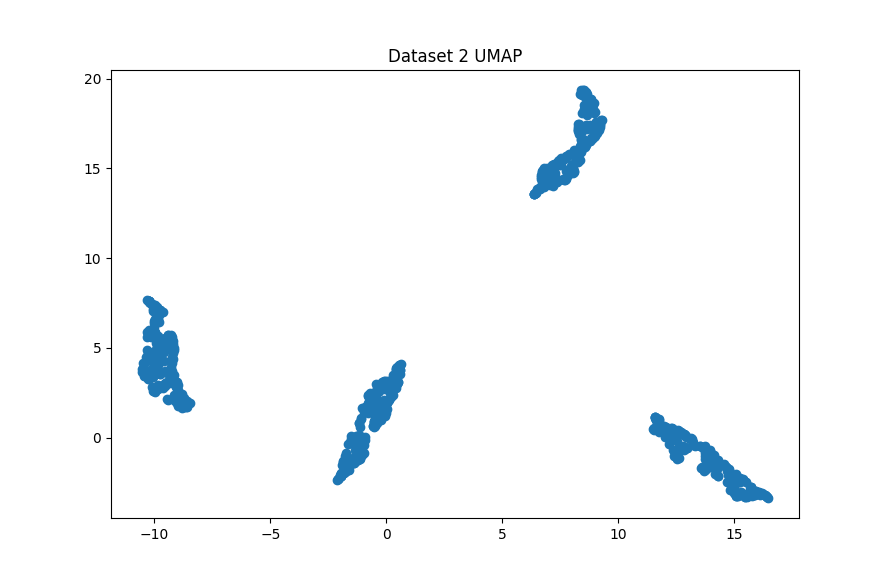
\includegraphics[scale=0.85]{dataset2_umap.png}
    \caption{Dataset 2 dimensionality reduction with UMAP}
\end{figure}

For dataset 2 however, optimum $K$ value obtained from elbow method and visualizations does not match with each other. According to t-SNE and UMAP visualizations 
there are 4 clusters. In contrary to 2D visualisations, elbow method suggest that optimum $K$ value is 3.

\subsection{Time Complexity Analysis}

Worst case time complexity of K-means is $O(kndi)$, where $k$ is the number of clusters, $n$ is the number of data samples, $d$ is the number of attributes, $i$ is the maximum number of iterations till convergence.
Worst case time complexity of K-medoid is worse than K-means since we have to iterate whole dataset once more to find data examples which minimizes loss. That means worst case time
complexity of K-medoids is $O(kn^2i)$. 

\section{Part 3}

\subsection{HAC}

\begin{figure}[H]
    \centering
    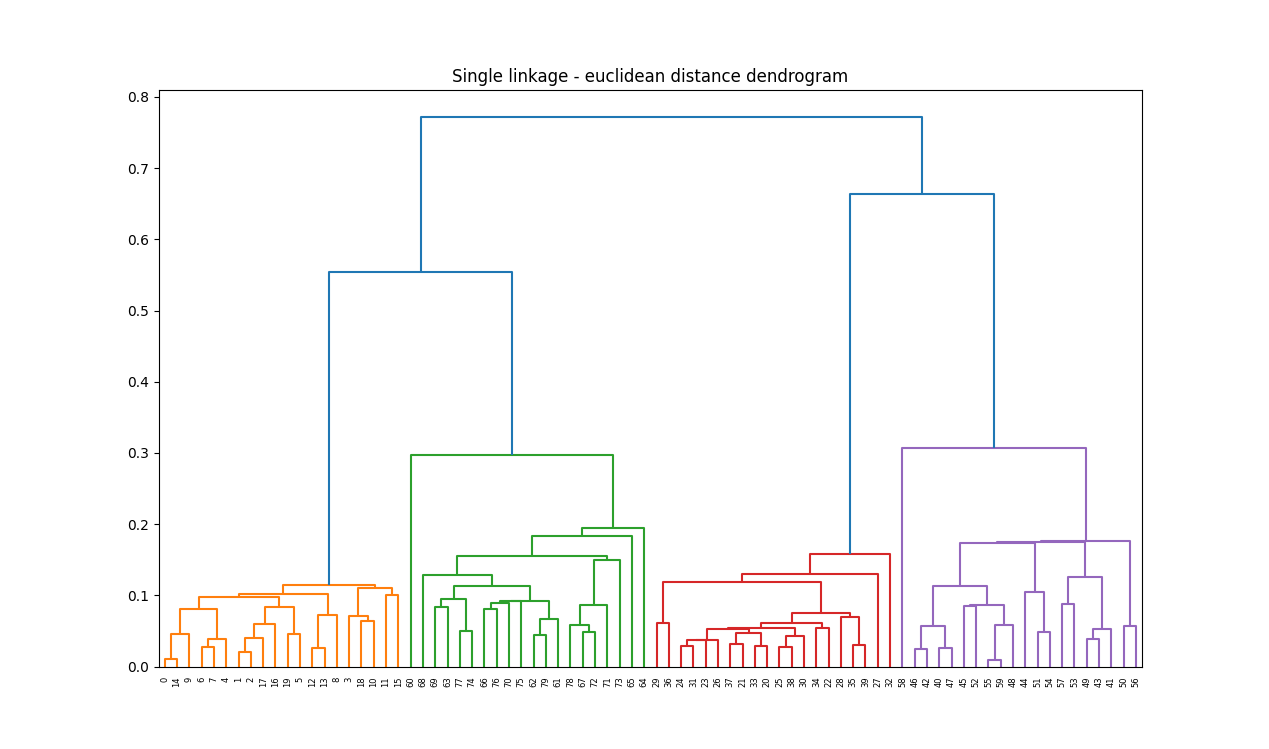
\includegraphics[scale=0.5]{single_euclidean_dendrogram.png}
    \caption{Dendrogram for single linkage - euclidean distance HAC}
\end{figure}

\begin{figure}[H]
    \centering
    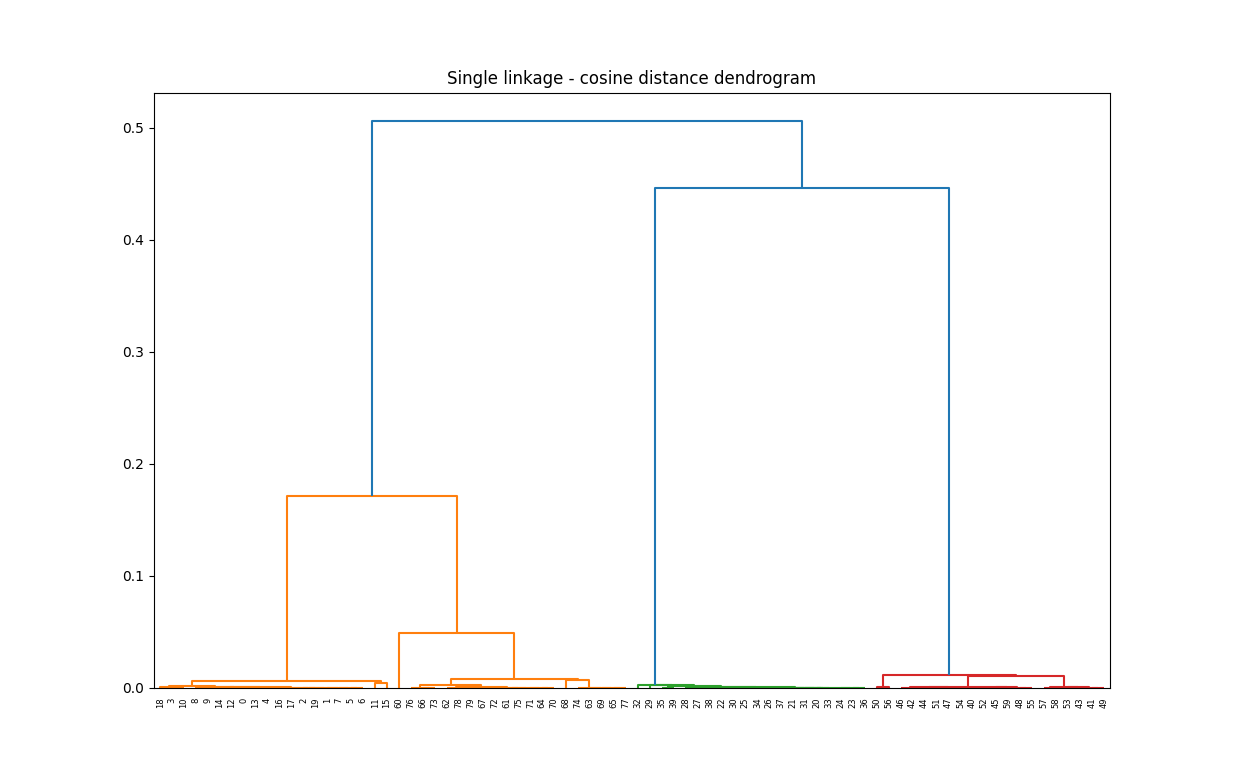
\includegraphics[scale=0.5]{single_cosine_dendrogram.png}
    \caption{Dendrogram for single linkage - cosine distance HAC}
\end{figure}

\begin{figure}[H]
    \centering
    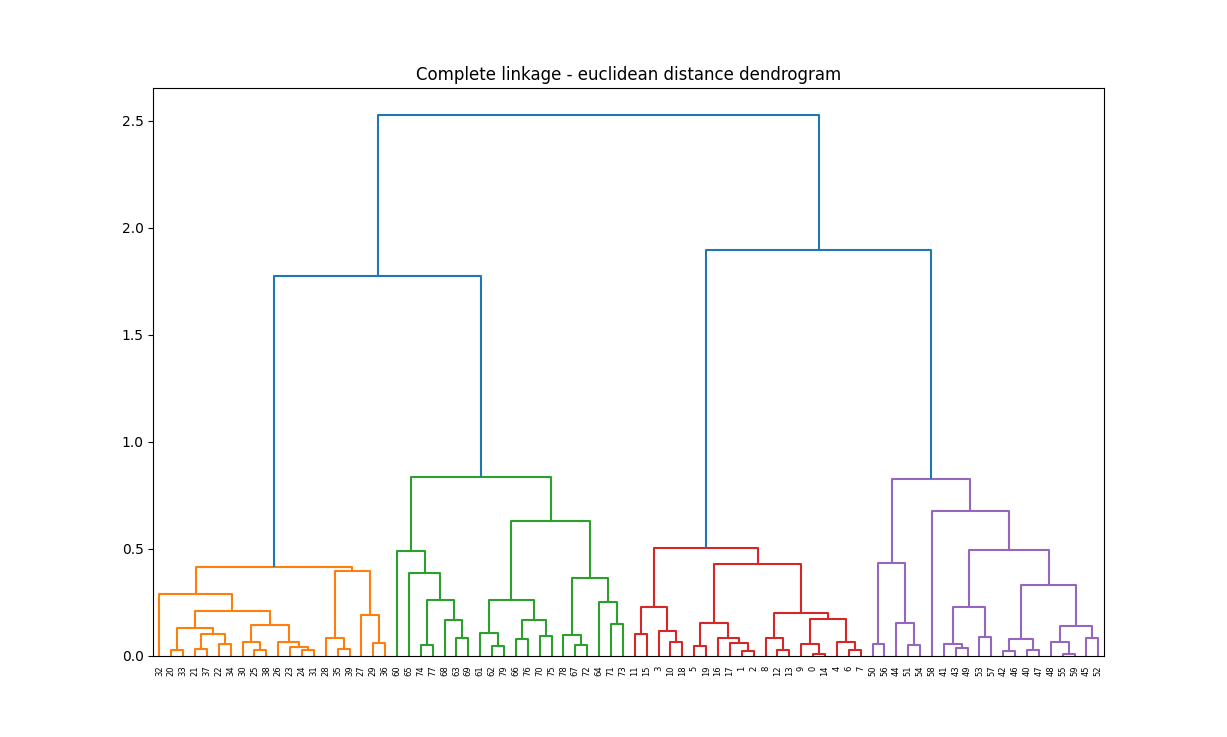
\includegraphics[scale=0.5]{complete_euclidean_dendrogram.png}
    \caption{Dendrogram for complete linkage - euclidean distance HAC}
\end{figure}

\begin{figure}[H]
    \centering
    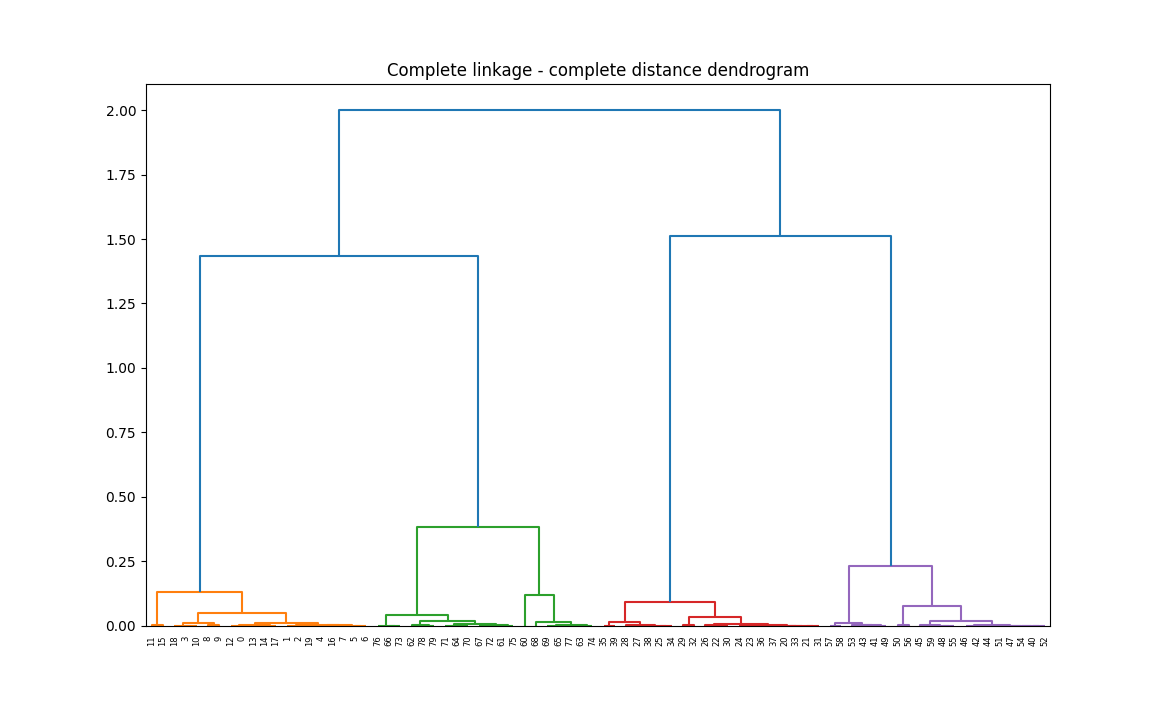
\includegraphics[scale=0.5]{complete_cosine_dendrogram.png}
    \caption{Dendrogram for complete linkage - cosine distance HAC}
\end{figure}

\begin{figure}[H]
    \centering
    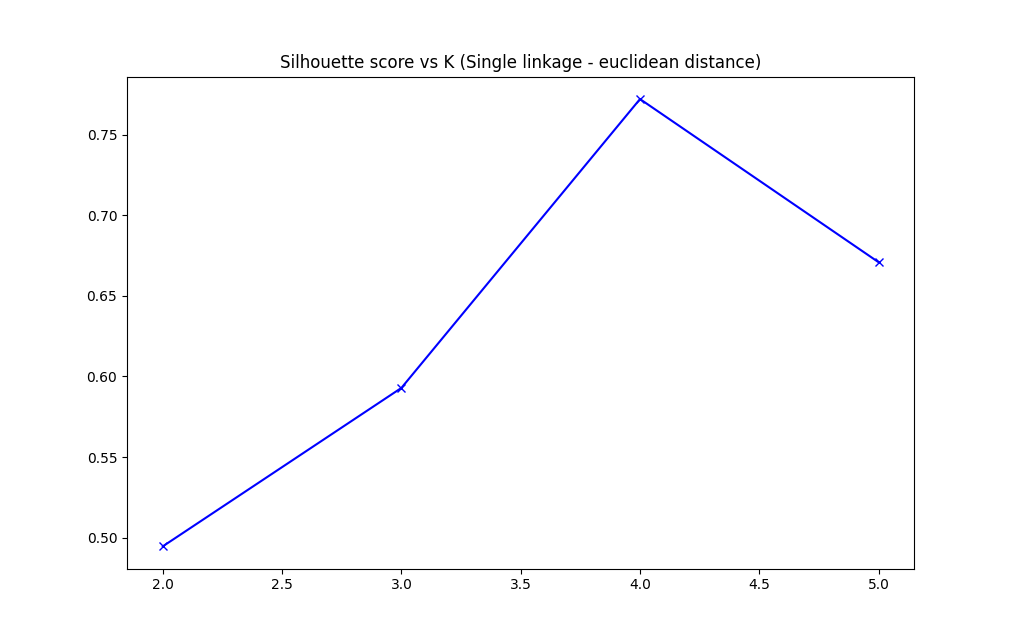
\includegraphics[scale=0.6]{single_euclidean_silh.png}
    \caption{Silhouette scores for single linkage - euclidean distance HAC}
\end{figure}

\begin{figure}[H]
    \centering
    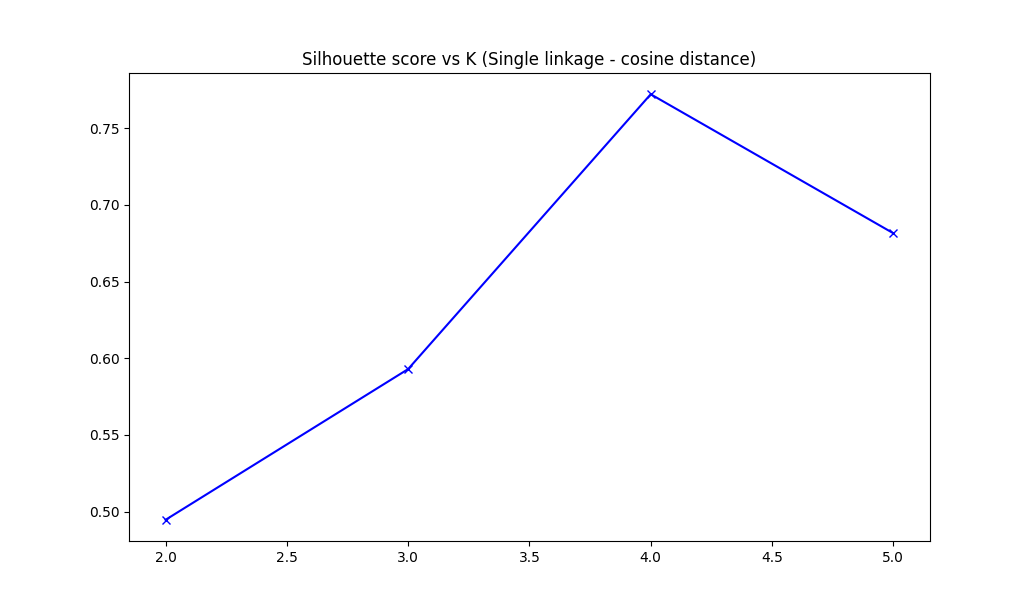
\includegraphics[scale=0.6]{single_cosine_silh.png}
    \caption{Silhouette scores for single linkage - cosine distance HAC}
\end{figure}

\begin{figure}[H]
    \centering
    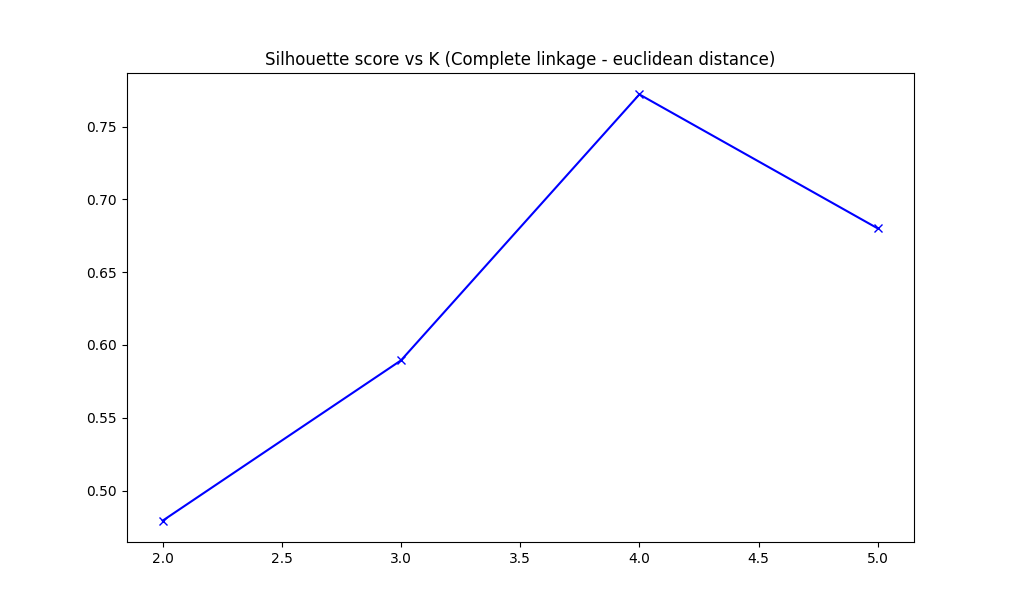
\includegraphics[scale=0.6]{complete_euclidean_silh.png}
    \caption{Silhouette scores for complete linkage - euclidean distance HAC}
\end{figure}

\begin{figure}[H]
    \centering
    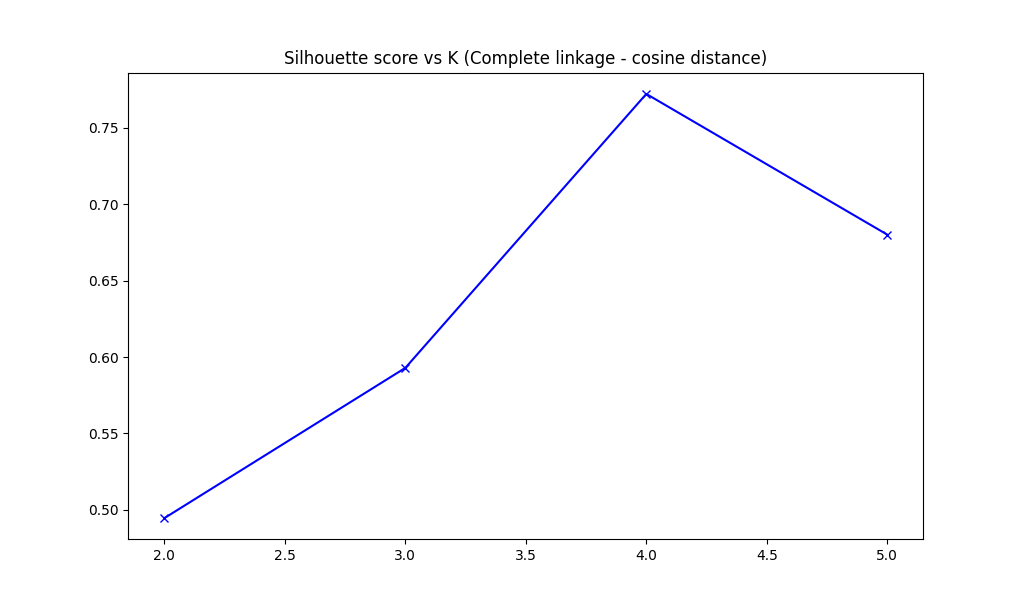
\includegraphics[scale=0.6]{complete_cosine_silh.png}
    \caption{Silhouette scores for complete linkage - cosine distance HAC}
\end{figure}

Best K value is $4$ for all of the configurations of HAC since it has the highest silhouette score for all of them.

\subsection{2D Visualisation}

\begin{figure}[H]
    \centering
    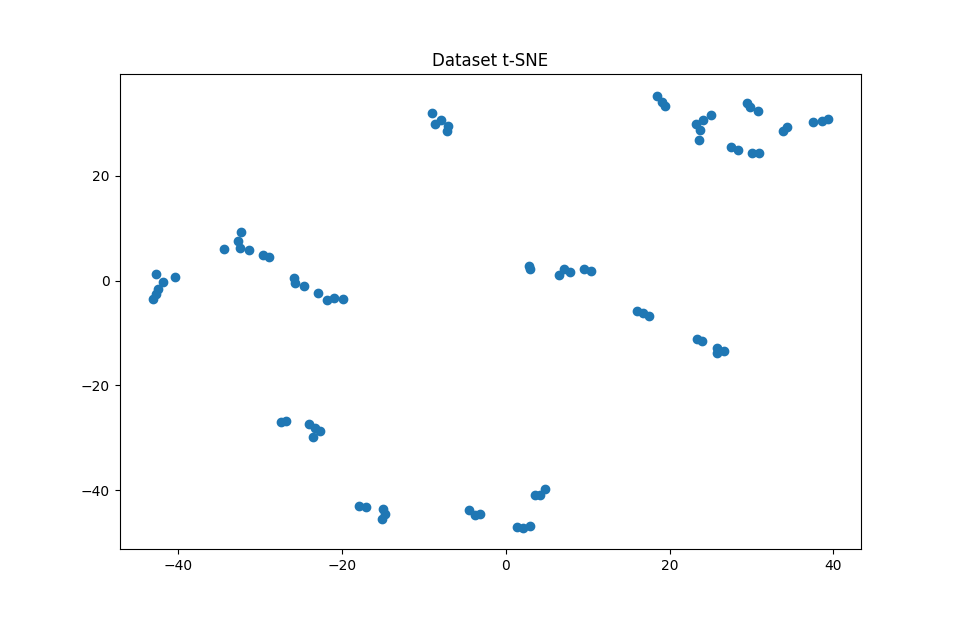
\includegraphics[scale=0.75]{hac_dataset_tsne.png}
    \caption{Dataset t-SNE reduction}
\end{figure}

\begin{figure}[H]
    \centering
    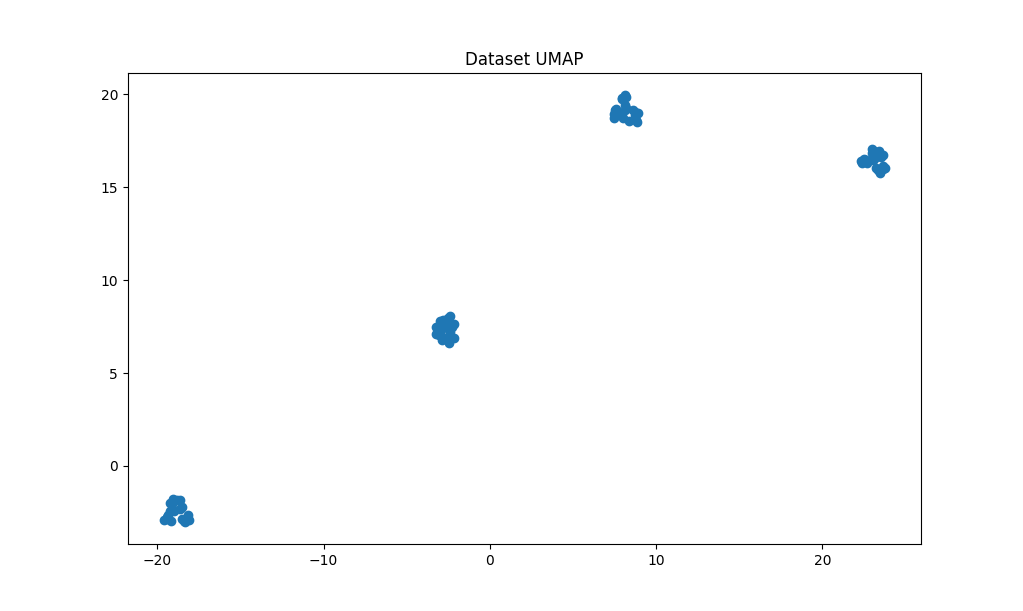
\includegraphics[scale=0.65]{hac_dataset_umap.png}
    \caption{Dataset UMAP reduction}
\end{figure}

Although clusters are not quite obvious in the t-SNE reduction graph, result of the UMAP reduction aligns with the silhouette score analysis. 
In the UMAP graph, it is obvious that there are 4 clusters.

\subsection{Time Complexity Analysis}

Worst case time complexity of the HAC is $O(n^3d)$, where $n$ is the number of data samples and $d$ is the number of attributes. Assuming that number of iterations $i$,
is not too large for K-means, I would prefer K-means to cluster dataset with large amount of samples.



\end{document}